% Ansatz.tex
\chapter{Eclipse Smarthome}
\label{chap:esh}
In diesem Kapitel wird \textit{Eclipse SmartHome} (ESH) vorgestellt. Es werden zunächst die grundlegenden Konzepte des Frameworks erläutert. Anschließend wird auf für die Arbeit relevante konkrete Aspekte näher eingegangen.

\section{Überblick}
Hier wird ein kurzer Überblick über Smarthome gegeben
- Was ist ESH?
- Zugrunde liegende Technologien
- Zentrale Features von ESH
- Wo kommt es zum Einsatz
-

Eclipse SmartHome positioniert sich als ein Framework, dass als Grundlage für die Entwicklung von konkreten SmartHome Endlösungen dienen soll. Tatsächlich kommt es in vielen bekannten Produkten zum Einsatz, wie z.B. openHAB und Qivicon. 


\subsubsection{Architektur}
Eclipse SmartHome hat eine serviceorientierte Architektur, basierend auf dem Java OSGi Framework. OSGi spezifiziert eine dynamische Softwareplattform, die hardwareunabhängig ist und es ermöglicht, Anwendungen zu modularisieren und zu verwalten. Der Funktionsweise der Kommunikation ist in Abbildung \ref{osgi:png} veranschaulicht.

\begin{figure}[h]
	\centering
	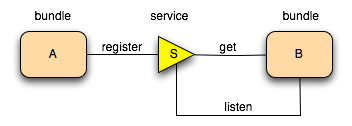
\includegraphics{bilder/osgi}
	\caption{OSGi Komponentenmodell: Kommunikation zwischen Bundles}
	\label{fig:osgi}
\end{figure}

Im Rahmen des OSGi Frameworks wird das gesamte Programm in verschiedene Softwarekomponenten (Bundles) aufgeteilt. Jede Komponente bietet und bezieht Services. Die angebotenen Services werden von den entsprechenden Bundles zur Laufzeit im System registriert, wonach andere Bundles, die diese Services beziehen, darüber informiert und ihrerseits gestartet werden können. Ein Bundle wird erst gestartet, wenn alle von ihm benötigten Services im System registriert wurden.\\

Ein derartiger modularer Aufbau erlaubt es verschiedene Bundles nahezu unabhängig von einander zu entwickeln und später einzelne Bundles gegen aktuellere Versionen problemlos auszutauschen. Eclipse SmartHome besteht derzeit aus über 130 solcher untereinander kommunizierender Softwarekomponenten.


\subsubsection{Features}
Trotz der Positionierung als Grundlage für konkrete Smart Home Lösungen anderer Anbieter, verfügt das Framework über den kompletten Service Stack, der in einem SmartHome zum Einsatz kommt. Es existiert ein Modellgerüst für die virtuelle Abbildung von realen Geräten. Für einige ausgewählte Geräte ist die Steuerung implementiert. Automatische Discovery von Geräten wird begrenzt unterstützt. Eine Rule Engine ist bereits integriert. Schließlich gibt es eine rudimentäre Benutzeroberfläche, die es erlaubt zur Laufzeit Geräte zum System hinzuzufügen und sie zu steuern. ESH hat eine ganze Reihe weiterer Features, wie z.B. Sprachunterstützung, die jedoch im Rahmen dieser Arbeit nicht von Interesse sind. 

Zentrales Prinzip des gesamten Frameworks ist es möglichst generische Schnittstellen zu definieren und exemplarische Implementierungen anzubieten, die die beabsichtigte Funktionsweise veranschaulichen. 

\\
Im Folgenden werden die verschiedenen Aspekte von ESH, die für die Arbeit relevant sind, erläutert.

\section{Modell}
Die virtuelle Abbildung der realen Geräte im System veranschaulicht Abbildung \ref{fig:esh_model}.

\begin{figure}[h]
	\centering
	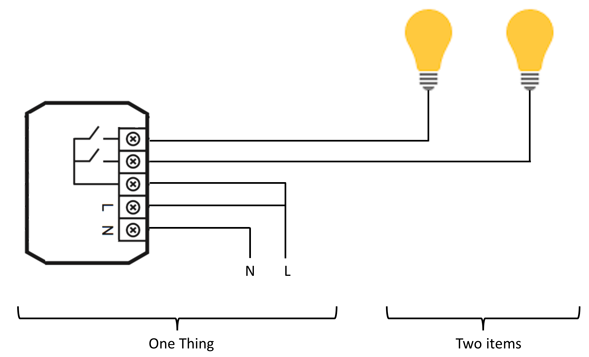
\includegraphics[width=\textwidth]{bilder/esh_model}
	\caption{Architektur von \textit{Things} und \textit{Items} in ESH}
	\label{fig:esh_model}
\end{figure}

\subsubsection{Things}
Things repräsentieren Entitäten, die zum System hinzugefügt werden können. In der Regel handelt es sich hierbei um verschiedene intelligente Geräte, wie beispielsweise eine \textit{Hue} Lampe oder eine Wetterstation. Derartige Geräte bieten eine oder mehrere Funktionalitäten über Channels an.

Things, die als Brücke zu anderen intelligenten Geräten dienen, werden als Bridges bezeichnet (z.B. \textit{Hue} Bridge);

\subsubsection{Channels}
Ein Channel stellt eine bestimmte Funktionalität eines Things dar. Things können eine beliebige Anzahl von Channels anbieten. Beispielsweise kann eine Hue Lampe einen einzigen \glqq Licht\grqq -Channel anbieten, während eine Wetterstation die Channels \glqq Temperatur\grqq , \glqq Druck\grqq{} und \glqq Feuchtigkeit\grqq unterstützt.

\subsubsection{Items}
Items repräsentieren konkrete, detaillierte Funktionalitäten eines Things. Beispielsweise kann ein Thing den Channel \glqq Licht\grqq{} unterstützen, wobei es 2 verschiedene Items besitzt, die beide jeweils eine physische Glühbirne verkörpern. Items haben einen Zustand, der im System gespeichert wird und können Commands empfangen.

\subsubsection{Links}
Links verbinden Items mit Things. Jeder Link assoziiert genau einen Channel des Things mit genau einem Item. Erst wenn ein Channel mit mindestens einem Item verbunden ist, gilt er als \glqq aktiviert\grqq{}. Channels und Items können über eine beliebige Anzahl von Links miteinander verbunden werden.


\subsection{Bindings}
Ein Binding ist eine Erweiterung (in der Regel ein eigenständiges Bundle) des Eclipse SmartHome Frameworks, dass für die Integration einer externen Funktionalität in Form von Things verantwortlich ist. 
In der Regel handelt es sich dabei um verschiedene intelligente Geräte, doch es können auch beispielsweise Webservices angebunden werden.

\subsection{Automatisierung}


\subsection{Deklarative Typen}
Eclipse SmartHome unterstützt die Möglichkeit, konkrete Typen durch die Sm

\subsection{Persistenz}
In Eclipse SmartHome ist eine MapDB\cite{•} bereits integriert. Dabei handelt es sich um eine leichtgewichtige, eingebettete Datenbank, in der zur Laufzeit alle Things, Items und Rules persistiert werden. 

%Move to entwurf?
Da im Rahmen dieser Arbeit es nur geringe Mengen an Daten bearbeitet werden müssen, ist es nicht notwendig, auf eine mächtigere Datenbank umzusteigen. Dadurch, dass die Webservices selbst als Things modelliert werden und alle notwendigen Konfigurationsdaten mit sich tragen, kann dieser Aspekt von ESH in seiner aktuellen Form wiederverwendet werden.



\section{Rule Engine}
\subsection{Triggers}
\subsection{Conditions}
\subsection{Actions}
\subsection{Events}

\section{Controller}
\subsection{Thing Handler}
Ein Binding besteht aus einer Reihe von Komponenten. Die grundlegenden Elemente sind im Folgenden aufgeführt:

\begin{enumerate}
\item Eine
\end{enumerate}

\subsection{Trigger/Action Handler}

\section{Fazit}
